% Provenance (never printed): see sources/outline_sources.md (Year 3:
% Glen's flow law; mass balance; ice sheets and ice shelves; sea ice;
% permafrost; the cryosphere's contribution to sea level).
% Brief: sources/book5/BRIEFS.md, ch. 24. Curves from figdata/bachelor-3/
% ice_flow.py (Glen slab, the plastic profile against the ETOPO1 Greenland
% transect, the Arkel ice cap) and sea_ice.py (NSIDC March and September
% extents, Stefan's law). Exercise and problem values in the Book 5 scratch
% calculator calc/ch24.py. The Arkel ice cap and the glaciers of the
% exercises are invented.
\chapter{Glaciología}\label{ch:b3:glaciology}

Se atraviesa Groenlandia de oeste a este siguiendo el paralelo \ang{72.5}N. El hielo
comienza a unas pocas decenas de kilómetros tierra adentro, asciende con fuerte pendiente y después cada vez más suavemente,
hasta una amplia cima de \qty{3229}{m} de altitud, y vuelve a descender hasta las montañas de la
costa oriental. Representada en una gráfica, la superficie se aproxima a una parábola tumbada,
con su vértice en el margen. Este capítulo muestra de dónde procede esa forma: de un material
que fluye cada vez más deprisa a medida que se le aplica un esfuerzo mayor, de modo que se
comporta casi como si no pudiera soportar más que cierto esfuerzo.
Después sigue el hielo desde la nieve que lo alimenta hasta el mar
que lo recibe.
% ledger: data:b5-etopo-greenland

\begin{recall}
Los glaciares, los casquetes de hielo, las plataformas de hielo, los icebergs, el hielo marino,
el permafrost y las edades de hielo figuran en los libros escolares. Las \omterm{def:b3:deformation-mechanisms:flow-law}{leyes de flujo} y la \omterm{def:b3:deformation-mechanisms:creep}{fluencia por dislocaciones} están en
el capítulo~\ref{ch:b3:deformation-mechanisms}; la \omterm{def:b3:gravity-geodesy:satgrav}{gravimetría por satélite} y el balance de masa
de los casquetes de hielo que mide en el capítulo~\ref{ch:b3:gravity-geodesy};
los testigos de hielo y sus isótopos de oxígeno, en el capítulo~\ref{ch:b3:stable-isotopes}.
El presupuesto del nivel del mar, la retroalimentación hielo--albedo y la subida del nivel
del mar por termoestérica están en el volumen de segundo año, en su capítulo sobre el cambio
climático antropogénico. El calor latente y la conducción de calor están en los libros de física.
\end{recall}

\section{El hielo como material}\label{sec:b3:glaciology:material}

El hielo glaciar es una roca, una masa de cristales de hielo entrelazados, y se deforma
cerca de su punto de fusión. Bajo un esfuerzo fluye por fluencia mediante el
movimiento de dislocaciones en sus cristales, como en las rocas
del capítulo~\ref{ch:b3:deformation-mechanisms}, y su \omterm{def:b3:deformation-mechanisms:flow-law}{ley de flujo} tiene la misma
forma: una potencia del esfuerzo multiplicada por un factor de Arrhenius.

\begin{theorem}[Ley de flujo de Glen]\label{thm:b3:glaciology:glen}
En el hielo glaciar isótropo, el tensor de velocidad de deformación es proporcional a la
parte desviadora del esfuerzo,
\[
\dot\varepsilon_{ij} = A(T)\,\tau_e^{\,n-1}\,\tau'_{ij}, \qquad
\tau_e^2 = \tfrac12\,\tau'_{ij}\tau'_{ij},
\]
con $n = 3$ y un \omterm{def:b3:glaciology:glen}{factor de velocidad} $A(T)$ que crece con la temperatura. En cizalla
simple, con $\tau_{xz}$ como única componente no nula de la parte desviadora del esfuerzo,
$\dot\varepsilon_{xz} = A\tau_{xz}^{\,n}$.
\end{theorem}
\index{ley de flujo de Glen}

\begin{proof}
La ley en sí es empírica: una ley de potencia ajustada a los experimentos de fluencia y a la
deformación de los glaciares, cuyo coeficiente y exponente se ajustan
conjuntamente. En cizalla simple $\tau'_{xz} = \tau'_{zx} = \tau_{xz}$ y las demás
componentes se anulan, así que $\tau_e^2 = \tfrac12(\tau_{xz}^2 +
\tau_{zx}^2) = \tau_{xz}^2$, y $\dot\varepsilon_{xz} = A\tau_{xz}^{\,n-1}
\tau_{xz}$.
\end{proof}
% ledger: pism:rheology

Con $n = 3$, el hielo es un fluido fuertemente no lineal: al duplicar el esfuerzo se deforma
ocho veces más deprisa. Su viscosidad efectiva, $1/(2A\tau_e^{\,2})$, no es una propiedad
del hielo por sí solo, sino que disminuye a medida que aumenta el esfuerzo.

\begin{definition}[Factor de velocidad (hielo)]\label{def:b3:glaciology:glen}
El \emph{factor de velocidad}\index{factor de velocidad (hielo)} $A(T)$ de la ley de Glen,
también llamado blandura del hielo, se escribe $A = A_0\exp(-Q/RT)$, con una energía de
activación $Q$. Un ajuste muy utilizado (Paterson y Budd) toma $A_0 =
\qty{3.61e-13}{s^{-1}.Pa^{-3}}$ y $Q = \qty{60}{kJ/mol}$ por debajo de
\qty{-10}{\celsius}, y $A_0 = \qty{1.73e3}{s^{-1}.Pa^{-3}}$ y $Q =
\qty{139}{kJ/mol}$ por encima de esa temperatura, más cerca del punto de fusión, donde el hielo
se ablanda más deprisa con la temperatura.
\end{definition}
% ledger: pism:rheology, codata:R

\begin{center}
\begin{tabular}{lccc}
\hline
temperatura & \qty{-25}{\celsius} & \qty{-10}{\celsius} & \qty{0}{\celsius}\\
$A$ (\unit{Pa^{-3}.yr^{-1}}) & \num{2.7e-18} & \num{1.4e-17} & \num{1.4e-16}\\
\hline
\end{tabular}
\end{center}

El hielo en su punto de fusión fluye unas cincuenta veces más deprisa que a
\qty{-25}{\celsius} bajo el mismo esfuerzo. Los esfuerzos en los glaciares son del
orden de un bar, \qty{e5}{Pa}.
% ledger: pism:rheology

Un glaciar se mueve de dos maneras. Su hielo se deforma por fluencia, en todas partes; y
donde el lecho está en el punto de fusión, puede además deslizarse.

\begin{definition}[Deslizamiento basal]\label{def:b3:glaciology:sliding}
El \emph{deslizamiento basal}\index{deslizamiento basal} es el movimiento de un glaciar sobre
su lecho, sobre una fina película de agua o una capa de sedimento blando y húmedo. Requiere un
lecho en el punto de fusión; un glaciar congelado a su lecho se mueve únicamente por la
fluencia de su hielo.
\end{definition}
% ledger: nsidc:glacier-flow

\section{Flujo glaciar}\label{sec:b3:glaciology:flow}

\begin{theorem}[Flujo de una losa de caras paralelas]\label{thm:b3:glaciology:slab}
Una losa de hielo de espesor $H$ y densidad $\rho$ descansa sobre un lecho de pendiente
$\alpha$ y fluye pendiente abajo por cizalla simple, deslizándose a la velocidad $u_b$. A una
altura $z$ sobre el lecho, el esfuerzo de cizalla es $\tau = \rho g(H - z)\sin\alpha$,
la velocidad
\[
u(z) = u_b + \frac{2A}{n + 1}(\rho g\sin\alpha)^n\left[H^{n+1} - (H -
z)^{n+1}\right],
\]
y el caudal por unidad de anchura $q = u_bH + \dfrac{2A}{n + 2}(\rho
g\sin\alpha)^nH^{n+2}$. El esfuerzo de cizalla basal es $\tau_b = \rho gH\sin\alpha$.
\end{theorem}

\begin{proof}
El hielo situado por encima de la altura $z$ tiene un peso $\rho g(H - z)$ por unidad de área; su
componente a lo largo de la pendiente, $\rho g(H - z)\sin\alpha$, se equilibra con el
esfuerzo de cizalla en su base, siendo la superficie libre de esfuerzo. Por la ley de Glen,
$\mathrm du/\mathrm dz = 2\dot\varepsilon_{xz} = 2A\tau^n$; integrando desde
el lecho, donde $u = u_b$, se obtiene $u(z)$, e integrando $u$ de 0 a $H$
se obtiene $q$.
\end{proof}

La velocidad cambia poco en la parte superior de la losa y es rápida cerca del lecho,
donde el esfuerzo es mayor: con $n = 3$ la cizalla se concentra en las capas más bajas.
La velocidad superficial crece como $H^{n+1} = H^4$ y como el cubo de la pendiente:
un glaciar dos veces más grueso fluye dieciséis veces más rápido.

\begin{definition}[Aproximación de hielo somero]\label{def:b3:glaciology:sia}
La \emph{aproximación de hielo somero}\index{aproximación de hielo somero} trata
un casquete de hielo cuyo espesor es pequeño frente a su anchura se trata localmente como
una losa de lados paralelos: en cada lugar el hielo se deforma por cizalla simple
bajo el \emph{esfuerzo motor} $\tau_d = \rho gH|\nabla s|$, siendo $s$ la
elevación de la superficie, y el caudal sigue la fórmula de la losa con el
espesor local y la pendiente superficial.
\end{definition}

En la \omterm{def:b3:glaciology:sia}{aproximación de hielo somero} el esfuerzo basal viene fijado por la forma
del hielo. Como la velocidad de deformación crece con el cubo del esfuerzo, un
aumento moderado del esfuerzo produce un gran aumento del flujo, que adelgaza el
hielo y vuelve a reducir el esfuerzo: el esfuerzo se mantiene dentro de un rango
estrecho, sea cual sea el tamaño de la masa de hielo. Llevado al límite, un material
que no se deforma en absoluto por debajo de un esfuerzo de fluencia $\tau_0$ y se
deforma sin límite por encima de él, y la forma se deduce.

\begin{proposition}[Perfil de un casquete de hielo plástico]\label{prop:b3:glaciology:nye}
Un casquete de hielo perfectamente plástico, de esfuerzo de fluencia $\tau_0$, sobre un
lecho plano y horizontal tiene, a la distancia $x$ hacia el interior desde su margen, la altura superficial
\[
h(x) = \sqrt{\frac{2\tau_0x}{\rho g}} .
\]
\end{proposition}
\index{perfil de un casquete de hielo plástico}

\begin{proof}
En todas partes el esfuerzo basal es igual al esfuerzo de fluencia: $\rho gh\,\mathrm
dh/\mathrm dx = \tau_0$, siendo la pendiente pequeña. Entonces $\mathrm d(h^2)/\mathrm
dx = 2\tau_0/(\rho g)$, y $h = 0$ en el margen.
\end{proof}

\begin{omfigure}
\begin{tikzpicture}
\begin{groupplot}[group style={group size=2 by 1, horizontal sep=1.5cm},
  height=0.4\linewidth,
  tick label style={font=\scriptsize}, label style={font=\small}, title style={font=\small}]
\nextgroupplot[width=0.38\linewidth, xlabel={$u/u_s$}, ylabel={altura sobre el lecho, $z/H$},
  xmin=0, xmax=1.05, ymin=0, ymax=1, title={una losa},
  legend style={font=\scriptsize, at={(0.03,0.97)}, anchor=north west}]
% computed in figdata/bachelor-3/ice_flow.py
\addplot[omThm, thick] table[x=u3, y=zeta] {figdata/out/bachelor-3-ice_flow-slab.dat};
\addlegendentry{$n = 3$}
\addplot[omDef, thick, densely dashed] table[x=u1, y=zeta] {figdata/out/bachelor-3-ice_flow-slab.dat};
\addlegendentry{$n = 1$}
\addplot[omMeth, thick] table[x=u3b, y=zeta] {figdata/out/bachelor-3-ice_flow-slab.dat};
\addlegendentry{$n = 3$, deslizamiento}
\nextgroupplot[width=0.58\linewidth, xlabel={distancia desde \ang{58}~O a lo largo de \ang{72.5}N (\unit{km})},
  ylabel={elevación (\unit{m})}, xmin=0, xmax=1270, ymin=-500, ymax=3700,
  title={Groenlandia}, scaled x ticks=false, xticklabel style={/pgf/number format/1000 sep={}},
  scaled y ticks=false, yticklabel style={/pgf/number format/1000 sep={}},
  legend style={font=\scriptsize, at={(0.5,0.03)}, anchor=south}]
\addplot[black, thin] table[x=x, y=h] {figdata/out/bachelor-3-ice_flow-gl.dat};
\addlegendentry{hielo y superficie del terreno}
\addplot[omThm, thick, densely dashed] table[x=x, y=h] {figdata/out/bachelor-3-ice_flow-nye-w.dat};
\addlegendentry{perfiles plásticos}
\addplot[omThm, thick, densely dashed, forget plot] table[x=x, y=h] {figdata/out/bachelor-3-ice_flow-nye-e.dat};
\draw[black!40] (axis cs:0,0) -- (axis cs:1270,0);
\node[font=\scriptsize, omThm, align=center] at (axis cs:330,2900) {$\tau_0 = $\\ \qty{72}{kPa}};
\node[font=\scriptsize, omThm, align=center] at (axis cs:1040,2900) {$\tau_0 = $\\ \qty{108}{kPa}};
\end{groupplot}
\end{tikzpicture}

\par\smallskip{\small A la izquierda, la velocidad a través de una losa de hielo, escalada por la
velocidad superficial: la ley de Glen ($n = 3$) concentra la cizalla cerca del lecho, un
fluido lineal ($n = 1$) la reparte; con deslizamiento todo el perfil se desplaza. A la
derecha, la superficie de Groenlandia a lo largo de \ang{72.5}N (ETOPO1 Ice
Surface, NOAA NCEI), y los perfiles plásticos ajustados a sus dos lados, para alturas
por encima de \qty{1000}{m} y un lecho situado al nivel del mar. Los ajustes requieren
esfuerzos de fluencia de \qty{72}{kPa} y \qty{108}{kPa}, del orden de un bar, como en los
glaciares reales; no reproducen los márgenes empinados, donde importan el lecho y la
fusión.}\label{fig:b3:glaciology:flow}
\end{omfigure}
% ledger: data:b5-etopo-greenland, pism:rheology

\section{Balance de masa}\label{sec:b3:glaciology:mass-balance}

Un glaciar se alimenta de nieve y pierde hielo por fusión, evaporación y, donde
alcanza el agua, por \omterm{def:b3:glaciology:grounding-line}{desprendimiento de icebergs}.
% ledger: nsidc:glacier-zones

\begin{definition}[Balance de masa; zonas de acumulación y de ablación; línea de equilibrio]\label{def:b3:glaciology:mass-balance}
El \emph{balance de masa del glaciar}\index{balance de masa del glaciar} es la variación
de la masa de un glaciar a lo largo de un año, expresada habitualmente en metros de
equivalente en agua promediados sobre su área. El \emph{balance de masa
superficial}\index{balance de masa superficial} es la parte debida a los procesos en
la superficie: la nevada menos la fusión, la escorrentía y la sublimación; el resto se
pierde por \omterm{def:b3:glaciology:grounding-line}{desprendimiento de icebergs} y por fusión en la base o bajo hielo flotante. La
\emph{zona de acumulación}\index{zona de acumulación} es la parte de la
superficie donde el balance de masa superficial a lo largo de un año es positivo; la
\emph{zona de ablación}\index{zona de ablación} la parte donde es negativo,
y la \emph{altitud de la línea de equilibrio}\index{altitud de la línea de equilibrio}
(ELA) la elevación de la línea que las separa, donde vale cero.
\end{definition}

\begin{omfigure}
\centering
\begin{tikzpicture}[>=stealth, font=\small, x=1cm, y=1cm]
% bed and surface of a valley glacier, long section
\fill[black!12] (0,0) -- (0,4.6) .. controls (2,3.6) and (6,1.4) .. (11,0) -- cycle;
\fill[omSea!45] (0,4.6) .. controls (2,3.6) and (6,1.4) .. (11,0)
  -- (11,0) .. controls (8,1.0) and (4,3.2) .. (0.6,5.4) -- (0,5.6) -- cycle;
\draw[thick, black!70] (0,4.6) .. controls (2,3.6) and (6,1.4) .. (11,0);
\draw[thick, omDef] (0,5.6) -- (0.6,5.4) .. controls (4,3.2) and (8,1.0) .. (11,0);
% equilibrium line
\draw[omThm, densely dashed, thick] (5.0,2.76) -- (5.0,4.6);
\node[omThm, font=\scriptsize, anchor=south] at (5.0,4.6) {línea de equilibrio (ELA)};
% balance arrows
\foreach \x/\y in {1.2/5.02, 2.4/4.27, 3.6/3.56} {\draw[->, omDef, thick] (\x,\y+0.55) -- (\x,\y+0.05);}
\foreach \x/\y in {6.4/2.02, 7.6/1.42, 8.8/0.86} {\draw[->, omThm, thick] (\x,\y+0.02) -- (\x,\y+0.52);}
\node[omDef, font=\scriptsize, align=center] at (2.4,6.2) {zona de acumulación:\\nieve incorporada};
\node[omThm, font=\scriptsize, align=center] at (8.6,2.5) {zona de ablación:\\hielo perdido};
% flow lines, computed inside the ice: buried in the accumulation zone, emerging in the ablation zone
\draw[->, black!60] plot[smooth] coordinates {(1.00,5.14) (1.98,4.28) (2.95,3.54) (3.93,2.93) (4.90,2.43) (5.88,2.00) (6.85,1.62) (7.83,1.24) (8.80,0.86)};
\draw[->, black!60] plot[smooth] coordinates {(2.20,4.39) (2.84,3.89) (3.48,3.43) (4.11,3.02) (4.75,2.67) (5.39,2.36) (6.03,2.08) (6.66,1.82) (7.30,1.56)};
\draw[->, black!60] plot[smooth] coordinates {(3.40,3.67) (3.74,3.44) (4.08,3.21) (4.41,3.00) (4.75,2.81) (5.09,2.63) (5.42,2.47) (5.76,2.32) (6.10,2.17)};
\node[font=\scriptsize, anchor=north east] at (10.9,-0.1) {frente glaciar};
\node[font=\scriptsize] at (3.0,1.4) {lecho rocoso};
\end{tikzpicture}

\par\smallskip{\small Esquema longitudinal de un glaciar de valle en
balance. Por encima de la línea de equilibrio, la nieve de cada año queda enterrada y
es arrastrada hacia el interior del glaciar; por debajo, la superficie pierde hielo cada año y
se renueva con hielo que asciende desde la profundidad. Las líneas de flujo (en gris) descienden en la
\omterm{def:b3:glaciology:mass-balance}{zona de acumulación} y ascienden en la \omterm{def:b3:glaciology:mass-balance}{zona de ablación}; el flujo lleva el
excedente de una zona al déficit de la otra.}\label{fig:b3:glaciology:zones}
\end{omfigure}
% ledger: nsidc:glacier-zones, nsidc:glacier-flow

En los casquetes de hielo y en los glaciares de alta montaña, la nieve no se convierte en hielo en una
sola estación. Queda enterrada por nieve posterior, se comprime y se recristaliza.

\begin{definition}[Neviza; cierre de los poros]\label{def:b3:glaciology:firn}
La \emph{neviza}\index{neviza} es nieve que ha sobrevivido al menos a una temporada de fusión
y que se va compactando hasta convertirse en hielo: más densa que la nieve, pero todavía permeable al aire.
El \emph{cierre de los poros}\index{cierre de los poros} es el punto de su
compactación, con una densidad de unos \qtyrange{820}{830}{kg/m^3}, en el que los poros
entre los granos quedan sellados en burbujas y el aire que contienen queda
aislado de la atmósfera.
\end{definition}

En los casquetes polares, el \omterm{def:b3:glaciology:firn}{cierre de los poros} se sitúa a \qtyrange{50}{120}{m} por debajo de la
superficie, según la temperatura, la acumulación y las
impurezas; el aire de las burbujas de un testigo de hielo es, por tanto, más joven que el
hielo que lo rodea, como recordó el Capítulo~\ref{ch:b3:stable-isotopes}. En la mayoría de los
glaciares, el paso de nieve a hielo tarda más de cien años.
% ledger: nsidc:firn, firn:close-off

Un glaciar no responde de inmediato a un cambio de su clima. Su espesor
debe cambiar antes de que su longitud pueda seguirlo.

\begin{proposition}[Tiempo de respuesta de un glaciar]\label{prop:b3:glaciology:response}
Un glaciar de espesor típico $H$ cuyo balance en el frente es $b_t <
0$ (en metros de hielo por año) se ajusta a un cambio de clima en un tiempo del
orden de
\[
\tau = \frac{H}{-b_t} .
\]
\end{proposition}

\begin{proof}
Un cambio del balance en $\delta b$ a lo largo del glaciar modifica su volumen
hasta que el área perdida o ganada en el frente, donde el balance es $b_t$, lo compensa:
$L\,\delta b = -b_t\,\delta L$ por unidad de anchura, para un glaciar
de longitud $L$. El cambio de volumen necesario es de unos $H\,\delta L$, y
el desequilibrio que lo impulsa es $L\,\delta b$ por año, al principio, de modo que el
cambio tarda $H\,\delta L/(L\,\delta b) = H/(-b_t)$ años.
\end{proof}

Un glaciar de \qty{200}{m} de espesor que pierde \qty{5}{m} de hielo al año en su
lengua necesita unos cuarenta años para responder. Por eso los glaciares van por detrás del
clima: los de hoy seguirán perdiendo masa durante décadas aunque la
temperatura deje de subir.
% ledger: ar6ch9:glaciers

\section{Casquetes de hielo y plataformas de hielo}\label{sec:b3:glaciology:ice-sheets}

Los casquetes de hielo de Groenlandia y de la Antártida contienen más del
\qty{99}{\percent} del hielo continental. El de Groenlandia cubre \qty{1.7}{\mega
km^2} y tiene un espesor máximo superior a \qty{3}{km}; el de la Antártida cubre
casi \qty{14}{\mega km^2} y tiene un espesor máximo de casi \qty{4.9}{km}. Muchas
zonas del casquete antártico descansan sobre un lecho situado por debajo del nivel del mar.
% ledger: nsidc:ice-sheets, ar6ch9:faq91

\begin{definition}[Corriente de hielo]\label{def:b3:glaciology:ice-stream}
Una \emph{corriente de hielo}\index{corriente de hielo} es una franja de un casquete de hielo que fluye
mucho más rápido que el hielo a ambos lados, principalmente por deslizamiento o por la
deformación de un lecho blando y húmedo, y drena hacia su margen una gran parte del
interior del casquete.
\end{definition}

\begin{definition}[Línea de apoyo; desprendimiento de icebergs]\label{def:b3:glaciology:grounding-line}
La \emph{línea de apoyo}\index{línea de apoyo} es la línea en la que el hielo
apoyado sobre su lecho empieza a flotar: mar afuera de ella, el hielo es una plataforma de hielo
o una lengua flotante de glaciar. El \emph{desprendimiento de icebergs}\index{desprendimiento de icebergs} es la rotura
de bloques de hielo, los icebergs, en el frente de un glaciar o de una plataforma de hielo
que termina en agua.
\end{definition}

Las plataformas de hielo flotan, de modo que su fusión no eleva el nivel del mar. Pero
están sujetas por sus laterales y por los umbrales del fondo marino donde encallan, y
el rozamiento que se produce allí se opone al flujo del hielo que hay detrás: lo
\emph{contienen}. Tras la desintegración de la plataforma de hielo Larsen~B en 2002, los
glaciares que la alimentaban se aceleraron hasta ocho veces.
% ledger: nsidc:ice-shelves

\begin{proposition}[Flotación]\label{prop:b3:glaciology:flotation}
Un hielo de densidad $\rho_i$ y espesor $H$ sobre un lecho situado a una profundidad $D$ bajo el
nivel del mar, en agua de mar de densidad $\rho_w$, flota si $H < (\rho_w/\rho_i)D$.
Con $\rho_i = \qty{917}{kg/m^3}$ y $\rho_w = \qty{1025}{kg/m^3}$, la \omterm{def:b3:glaciology:grounding-line}{línea de apoyo} se sitúa donde el
hielo tiene un espesor de $1.12\,D$.
\end{proposition}

\begin{proof}
El hielo flotante desplaza un peso de agua igual al suyo propio: una columna de espesor $H$
necesita un calado de $\rho_iH/\rho_w$. Si el agua es más profunda que ese calado,
el hielo flota.
\end{proof}
% ledger: iapws:ice-density, noaa:seawater-1025

\begin{omfigure}
\centering
\begin{tikzpicture}[>=stealth, font=\small, x=1cm, y=1cm]
% sea and bed
\fill[omSea!50] (4.2,0) rectangle (11,-2.8);
\fill[black!15] (0,-0.9) -- (2.2,-2.0) -- (4.6,-1.6) -- (7.0,-2.3) -- (11,-2.6)
  -- (11,-3.2) -- (0,-3.2) -- cycle;
\draw[thick, black!60] (0,-0.9) -- (2.2,-2.0) -- (4.6,-1.6) -- (7.0,-2.3) -- (11,-2.6);
% grounded ice and ice shelf
\fill[white] (0,-0.9) -- (0,2.4) .. controls (2,2.2) and (3.6,1.4) .. (4.6,0.2)
  -- (9.2,0.12) -- (9.2,-1.0) -- (4.6,-1.6) -- (2.2,-2.0) -- cycle;
\draw[thick, omDef] (0,2.4) .. controls (2,2.2) and (3.6,1.4) .. (4.6,0.2) -- (9.2,0.12)
  -- (9.2,-1.0) -- (4.6,-1.6);
\draw[thick] (0,0) -- (0,0);
\draw[omDef!60, thin] (0,0) -- (4.3,0); \draw[omDef!60, thin] (9.2,0) -- (11,0);
\node[font=\scriptsize, anchor=south west] at (0.05,0.02) {nivel del mar};
% icebergs
\fill[white] (10.1,0.1) rectangle (10.6,-0.7); \draw[omDef] (10.1,0.1) rectangle (10.6,-0.7);
% labels
\fill[omThm] (4.6,-1.6) circle (0.07);
\draw[omThm, ->] (4.0,-2.6) node[anchor=north, font=\scriptsize] {línea de apoyo} -- (4.55,-1.68);
\node[font=\scriptsize] at (1.4,1.1) {casquete de hielo apoyado};
\node[font=\scriptsize] at (6.9,-0.7) {plataforma de hielo flotante};
\node[font=\scriptsize, anchor=south] at (9.2,0.2) {frente de desprendimiento};
\node[font=\scriptsize, anchor=north, align=center] at (10.35,-0.8) {iceberg};
\node[font=\scriptsize, align=center] at (2.1,-2.55) {el lecho se profundiza\\hacia el interior};
\draw[->, black!60, thick] (2.2,1.6) -- (3.6,1.0);
\draw[->, black!60, thick] (5.4,-0.2) -- (7.0,-0.2);
\node[font=\scriptsize, align=center, omMeth] at (7.0,1.2) {contención: rozamiento en los\\laterales de la plataforma y en los umbrales apoyados};
\draw[->, omMeth, thick] (7.6,0.6) -- (6.6,0.6);
\end{tikzpicture}

\par\smallskip{\small Esquema de una sección de un casquete de hielo marino, no a
escala. El hielo descansa sobre un lecho por debajo del nivel del mar, que se profundiza hacia el interior; en la
\omterm{def:b3:glaciology:grounding-line}{línea de apoyo} empieza a flotar, como plataforma de hielo, que pierde hielo por
desprendimiento en su frente y por fusión desde abajo. El rozamiento en la plataforma donde
queda retenida por sus laterales y por los umbrales del fondo marino, se opone al flujo del
hielo apoyado.}\label{fig:b3:glaciology:grounding}
\end{omfigure}
% ledger: nsidc:ice-shelves, ar6ch9:misi

En un lecho que se profundiza hacia el interior la \omterm{def:b3:glaciology:grounding-line}{línea de apoyo} es frágil. Donde el
agua es más profunda, el hielo en la \omterm{def:b3:glaciology:grounding-line}{línea de apoyo} es más grueso, por la condición de
flotación, y por el teorema de la losa el flujo de una columna más gruesa crece
con fuerza con su espesor. Si la \omterm{def:b3:glaciology:grounding-line}{línea de apoyo} retrocede por una pendiente de este
tipo, alcanza hielo más grueso que descarga más, adelgaza más deprisa y permite que la
línea retroceda aún más.

\begin{definition}[Inestabilidad de los casquetes de hielo marinos]\label{def:b3:glaciology:misi}
La \emph{inestabilidad de los casquetes de hielo marinos}\index{inestabilidad de los casquetes de hielo marinos}
(MISI) es el retroceso autorreforzado propuesto de la \omterm{def:b3:glaciology:grounding-line}{línea de apoyo} de un
casquete de hielo que descansa sobre un lecho que desciende hacia el interior: sin
la contención de una plataforma de hielo, la \omterm{def:b3:glaciology:grounding-line}{línea de apoyo} en un lecho de este tipo es
intrínsecamente inestable hasta que alcanza un lecho que asciende.
\end{definition}

Las plataformas de hielo pueden mantener la \omterm{def:b3:glaciology:grounding-line}{línea de apoyo} en su lugar incluso en una pendiente descendente.
Los modelos en los que se eliminan todas las plataformas de hielo antárticas y no se les permite
reformarse pierden hielo equivalente a \qtyrange{2}{10}{m} de nivel del mar en 500
años por medio de esta inestabilidad, \qtyrange{2}{5}{m} de ellos procedentes de la
Antártida Occidental. En los casquetes de hielo que descansan sobre todo sobre lecho rocoso por encima del nivel del mar, como
Groenlandia, el proceso autorreforzado principal es otro: a medida que la superficie
se funde y desciende, queda en aire más cálido y se funde más.
% ledger: ar6ch9:misi, ar6ch9:faq91

\begin{definition}[Equivalente en nivel del mar]\label{def:b3:glaciology:sle}
El \emph{equivalente en nivel del mar}\index{equivalente en nivel del mar} de una masa de
hielo continental es la subida del nivel medio global del mar que causaría su fusión
si el agua se extendiera sobre el océano actual.
\end{definition}

\begin{proposition}[Equivalente en nivel del mar de una masa de hielo]\label{prop:b3:glaciology:sle}
Una masa $M$ de hielo que descansa por encima del nivel del mar, extendida sobre un océano de área
$A_o$ como agua de densidad $\rho_w$, eleva el nivel del mar en $M/(\rho_wA_o)$:
unos \qty{1}{mm} por cada \qty{360}{Gt}.
\end{proposition}

\begin{proof}
El agua ocupa el volumen $M/\rho_w$ sobre el área $A_o$. Con las
\qty{360}{Gt} por milímetro adoptadas por las evaluaciones del balance de masa de los
casquetes de hielo, $A_o\rho_w = \qty{3.6e17}{kg/m}$: un océano de unos
\qty{3.6e8}{km^2} para agua con la densidad del agua dulce.
\end{proof}
% ledger: data:b5-imbie

El hielo que ya está por debajo del nivel del mar desplaza agua de mar, de modo que cuenta menos:
los \qty{30}{\mega km^3} de hielo de la Antártida equivalen a unos
\qty{58}{m} de nivel del mar, menos que su masa dividida por
\qty{360}{Gt/mm}.
% ledger: nsidc:ice-sheets

\begin{omfigure}
\centering
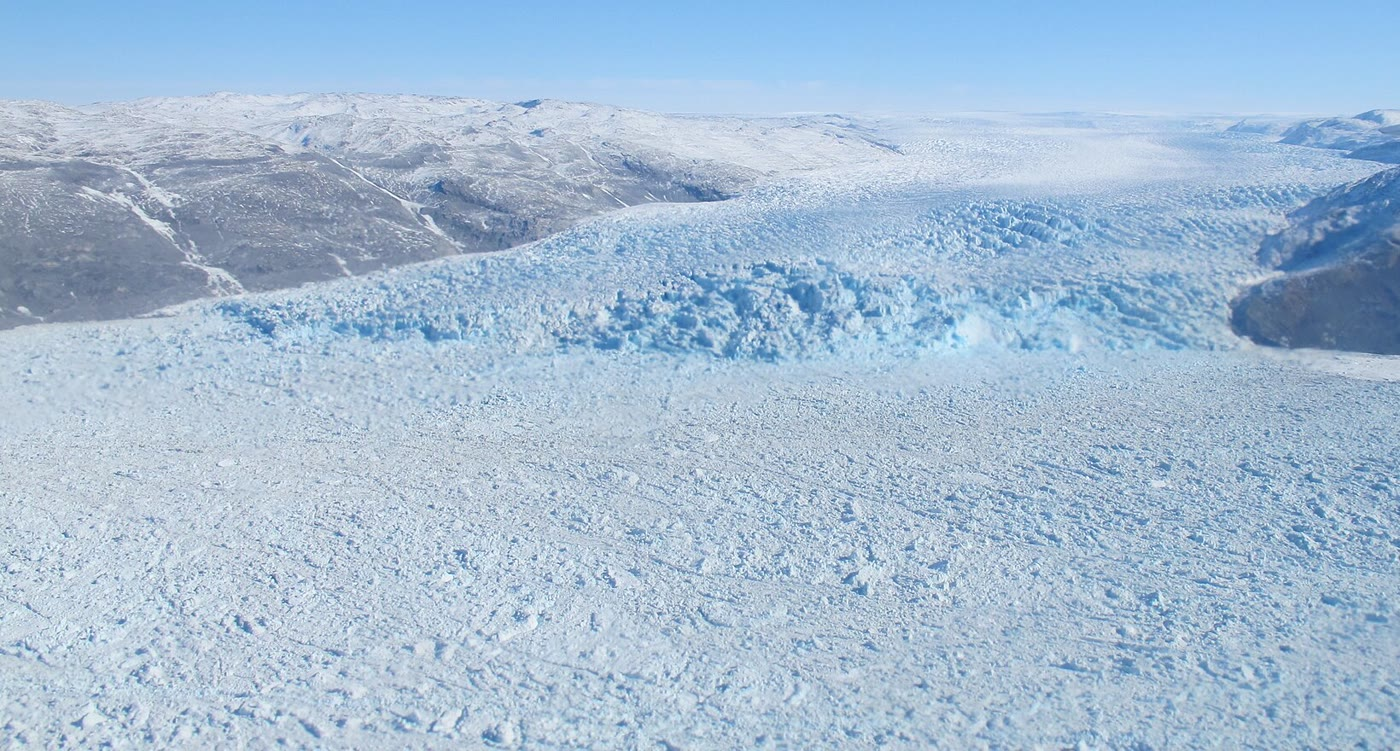
\includegraphics[width=0.82\linewidth]{images/book5/b3-greenland-outlet.jpg}

\par\smallskip{\small Un glaciar de desagüe del casquete de hielo de Groenlandia,
entre montañas, que termina en el mar en su frente de desprendimiento; la pared rota
de hielo azul que atraviesa el centro de la imagen; el fiordo situado delante está colmatado
de hielo desprendido y de hielo marino. Fotografiado desde una aeronave de la NASA
Operation IceBridge en abril de 2014 (NASA / Jim Yungel, dominio
público).}\label{fig:b3:glaciology:outlet}
\end{omfigure}
% ledger: photo:b3-greenland-outlet

\begin{inthefield}[Un campamento sobre el hielo]
\begin{minipage}[t]{0.55\linewidth}\vspace{0pt}
En un casquete de hielo los instrumentos de los glaciólogos se desplazan en trineo y
se alojan en tiendas. Para medir con qué rapidez se mueve el hielo, congelan un poste en la
nieve y montan sobre él la antena de un receptor de navegación por satélite. Los
receptores empleados en geodesia fijan una posición con un margen de unos pocos centímetros, de modo que
las posiciones repetidas a lo largo de semanas o de estaciones dan la velocidad y la dirección
del hielo, y la altura del poste, medida de nuevo, la reducción o el
aumento del espesor del hielo situado debajo.
\end{minipage}\hfill
\begin{minipage}[t]{0.42\linewidth}\vspace{0pt}
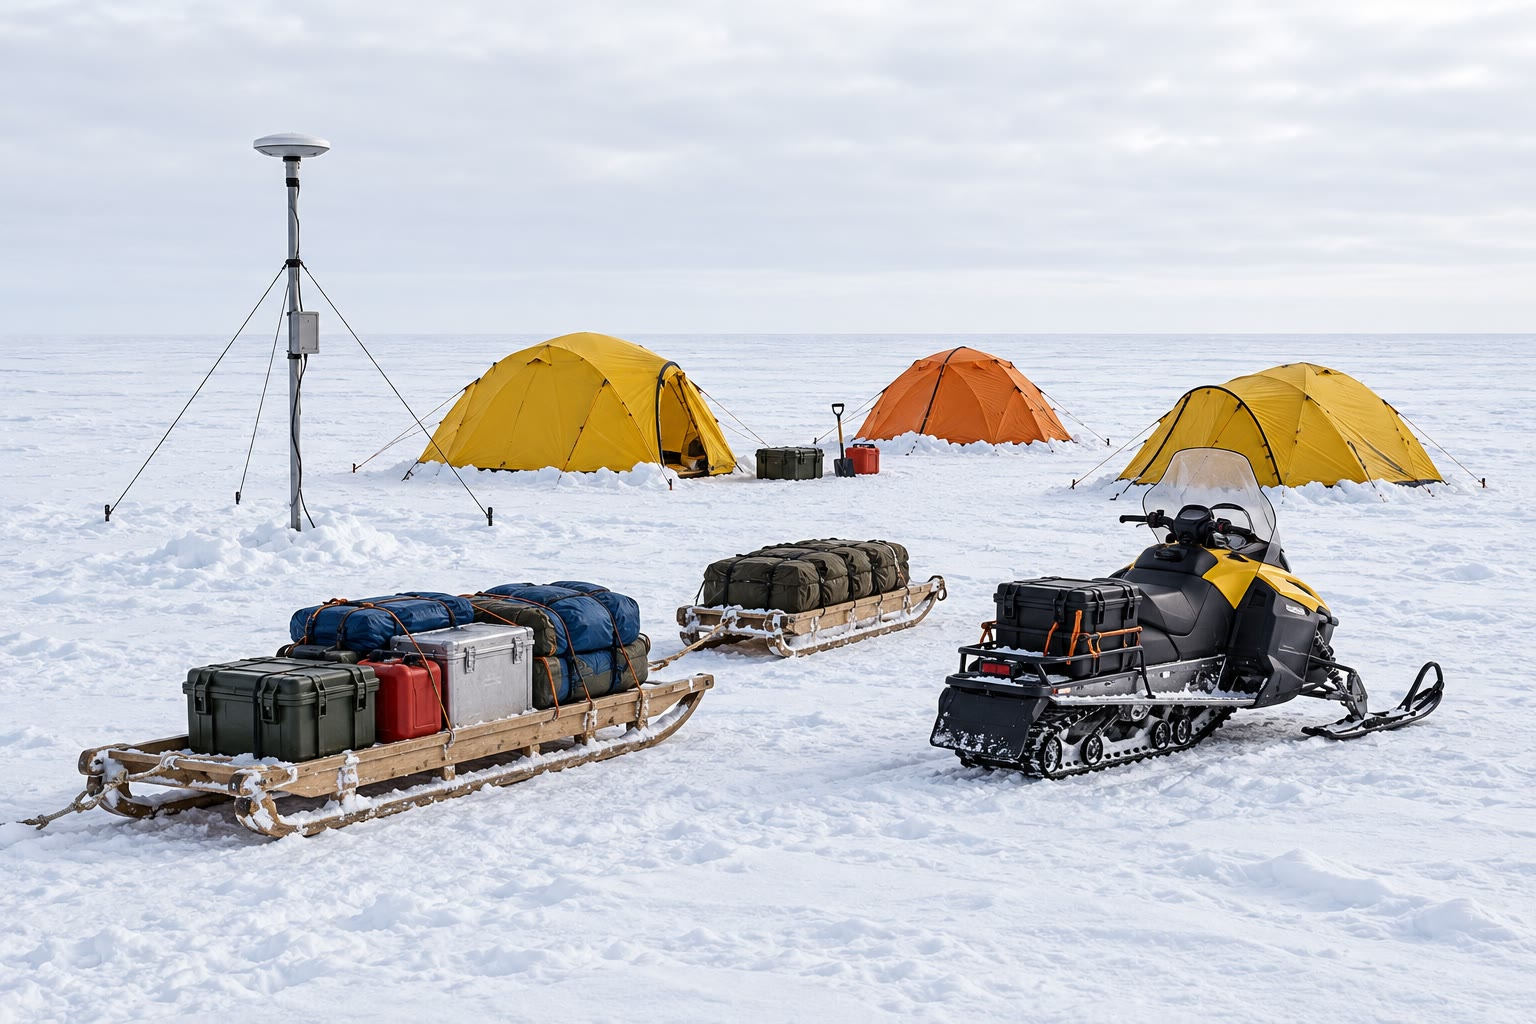
\includegraphics[width=\linewidth]{images/book5/ai/b3-glaciology-camp.jpg}

{\scriptsize Un campamento de campo sobre un casquete de hielo: tiendas, trineos y una
moto de nieve, y una antena de navegación por satélite sobre un mástil sujeto por
cables tensores (Ilustración generada por IA.)}
\end{minipage}
\end{inthefield}
% ledger: gps:high-end

\section{Hielo marino y permafrost}\label{sec:b3:glaciology:sea-ice}

El hielo marino se forma, crece y se funde en el océano. En el Ártico alcanza su
área máxima en marzo y su área mínima en septiembre.
% ledger: nsidc:sea-ice-def

\begin{definition}[Extensión del hielo marino]\label{def:b3:glaciology:sea-ice}
La \emph{extensión del hielo marino}\index{extensión del hielo marino} es el área total de las
celdas de un mapa satelital en las que el hielo marino cubre más de
\qty{15}{\percent} de la superficie. Es mayor que el área del hielo marino,
que cuenta solo el propio hielo.
\end{definition}
% ledger: nsidc:sea-ice-def

Desde que los satélites comenzaron a cartografiarla en 1979, la extensión ártica se ha reducido,
en marzo y mucho más en septiembre: a razón de \qty{0.74}{\mega km^2} por década en
septiembre, unos \qty{12}{\percent} de la media de 1981--2010 por década, frente a
\qty{0.38}{\mega km^2}, \qty{2.5}{\percent}, en marzo. La extensión mínima
de septiembre registrada hasta ahora, \qty{3.57}{\mega km^2}, se produjo en 2012. El hielo marino
ártico refleja de \qtyrange{50}{70}{\percent} de la luz solar, y el océano abierto,
unos \qty{6}{\percent}: la pérdida del hielo oscurece la superficie, la
retroalimentación hielo--albedo del volumen de segundo año.
% ledger: data:b5-nsidc-extent, nsidc:sea-ice-reflect

El hielo marino crece por su base, donde el agua de mar se congela sobre él, y el calor latente
de esa congelación debe conducirse hacia arriba a través del hielo hasta el aire frío.

\begin{theorem}[Ley de Stefan]\label{thm:b3:glaciology:stefan}
Un hielo marino de conductividad térmica $k_i$, densidad $\rho_i$ y calor latente de
fusión $L$, con su superficie mantenida a una temperatura $\Delta T$ por debajo del
punto de congelación del agua subyacente, crece, si el calor procedente del océano es
despreciable, según
\[
h(t)^2 - h(0)^2 = \frac{2k_i\,\Delta T}{\rho_iL}\,t .
\]
Bajo una capa de nieve de espesor $h_s$ y conductividad $k_s$ la velocidad de crecimiento
es $\mathrm dh/\mathrm dt = \Delta T/[\rho_iL(h/k_i + h_s/k_s)]$.
\end{theorem}

\begin{proof}
La temperatura en el hielo delgado es lineal, desde el punto de congelación en la base
hasta la temperatura de la superficie en la parte superior, de modo que el flujo de calor a través de él es
$k_i\Delta T/h$, o, a través de hielo y nieve en serie, $\Delta T/(h/k_i +
h_s/k_s)$. La congelación de una capa $\mathrm dh$ libera $\rho_iL\,\mathrm dh$ por
unidad de área, que este flujo debe evacuar: $\rho_iL\,\mathrm dh/\mathrm dt
= k_i\Delta T/h$. Entonces $\mathrm d(h^2)/\mathrm dt = 2k_i\Delta T/(\rho_iL)$.
\end{proof}

Con $k_i = \qty{2.03}{W.m^{-1}.K^{-1}}$, $L = \qty{3.34e5}{J/kg}$ y
$\rho_i = \qty{917}{kg/m^3}$, una superficie \qty{20}{K} por debajo del punto de congelación
forma \qty{1.5}{m} de hielo en cien días y \qty{2.1}{m} en doscientos.
La nieve, con una conductividad de \qty{0.30}{W.m^{-1}.K^{-1}}, es un buen
aislante: \qty{20}{cm} de ella reducen a menos de la mitad el crecimiento. El hielo grueso crece
despacio, el hielo delgado rápidamente: la ley tiende a igualar el espesor del hielo
tras un verano de fusión.
% ledger: cice:constants, iapws:ice-density

\begin{omfigure}
\begin{tikzpicture}
\begin{groupplot}[group style={group size=2 by 1, horizontal sep=1.5cm},
  width=0.48\linewidth, height=0.4\linewidth,
  tick label style={font=\scriptsize}, label style={font=\small}, title style={font=\small}]
\nextgroupplot[xlabel={año}, ylabel={extensión (\unit{\mega km^2})}, xmin=1977, xmax=2028,
  ymin=0, ymax=18, title={Extensión del hielo marino ártico},
  xticklabel style={/pgf/number format/1000 sep={}},
  legend style={font=\scriptsize, at={(0.03,0.66)}, anchor=west}]
% computed in figdata/bachelor-3/sea_ice.py
\addplot[omDef, thick, mark=*, mark size=0.9pt] table[x=year, y=mar] {figdata/out/bachelor-3-sea_ice-extent.dat};
\addlegendentry{marzo}
\addplot[omThm, thick, mark=*, mark size=0.9pt] table[x=year, y=sep] {figdata/out/bachelor-3-sea_ice-extent.dat};
\addlegendentry{septiembre}
\addplot[black!60, densely dashed, forget plot] table[x=year, y=mar] {figdata/out/bachelor-3-sea_ice-trend.dat};
\addplot[black!60, densely dashed, forget plot] table[x=year, y=sep] {figdata/out/bachelor-3-sea_ice-trend.dat};
\nextgroupplot[xlabel={días de congelación}, ylabel={espesor del hielo (\unit{m})}, xmin=0, xmax=200,
  ymin=0, ymax=2.4, title={crecimiento, $\Delta T = \qty{20}{K}$},
  legend style={font=\scriptsize, at={(0.97,0.03)}, anchor=south east}]
\addplot[omMeth, thick] table[x=day, y=h0] {figdata/out/bachelor-3-sea_ice-stefan.dat};
\addlegendentry{hielo desnudo}
\addplot[omDef, thick, densely dashed] table[x=day, y=hs] {figdata/out/bachelor-3-sea_ice-stefan.dat};
\addlegendentry{bajo \qty{20}{cm} de nieve}
\end{groupplot}
\end{tikzpicture}

\par\smallskip{\small A la izquierda, la \omterm{def:b3:glaciology:sea-ice}{extensión media del hielo marino} ártico en marzo y en
septiembre, 1979--2026 (NSIDC Sea Ice Index, versión~4), con
tendencias por mínimos cuadrados (discontinuas): \qty{-0.38}{\mega km^2} y \qty{-0.74}{\mega km^2} por
década. A la derecha, el crecimiento del hielo marino por conducción bajo una superficie
\qty{20}{K} por debajo del punto de congelación, sin calor oceánico: hielo desnudo según la ley de Stefan,
y el mismo hielo bajo \qty{20}{cm} de nieve.}\label{fig:b3:glaciology:sea-ice}
\end{omfigure}
% ledger: data:b5-nsidc-extent, cice:constants

El permafrost es el terreno que se mantiene a \qty{0}{\celsius} o por debajo durante dos años
o más. Se extiende bajo cerca de una cuarta parte de la tierra emergida del
hemisferio norte.
% ledger: nsidc:permafrost

\begin{definition}[Capa activa]\label{def:b3:glaciology:permafrost}
La \emph{capa activa}\index{capa activa} es la capa de terreno situada sobre
el permafrost que se funde cada verano y vuelve a congelarse cada invierno.
\end{definition}

Su espesor está determinado, como el crecimiento del hielo marino, por la conducción de calor
hacia el terreno durante la temporada de deshielo, frente al calor latente del
hielo del terreno. Las temperaturas del permafrost han aumentado en las últimas tres o
cuatro décadas en todas las regiones con permafrost (confianza alta);
el permafrost se ha calentado a escala mundial \qty{0.29}{\celsius} [\numrange{0.17}{0.41}]
entre 2007 y 2016 (confianza media), y el aumento del
espesor de la \omterm{def:b3:glaciology:permafrost}{capa activa} es un fenómeno panártico (confianza media).
Donde su hielo se funde, el terreno puede colapsar.
% ledger: ar6ch9:permafrost, nsidc:permafrost-thaw

\section{La criosfera y el nivel del mar}\label{sec:b3:glaciology:sea-level}

El balance del nivel del mar del volumen de segundo año suma la expansión del océano que se
calienta al agua aportada por el hielo y por la tierra. De los
\qty{3.69}{mm/yr} de subida del nivel del mar observados entre 2006 y 2018, los glaciares
aportaron \qty{0.62}{mm/yr}, Groenlandia \qty{0.63}{mm/yr} y la Antártida
\qty{0.37}{mm/yr}: en conjunto, el hielo aportó más que la expansión del océano,
\qty{1.39}{mm/yr}.
% ledger: ar6ch9:table95

\begin{dated}{2021}
Groenlandia perdió \qty{4890}{Gt} de hielo entre 1992 y 2020 [4140 a 5640],
\qty{13.5}{mm} de nivel del mar, a un ritmo que pasó de \qty{39}{Gt/yr} en los
años noventa a \qty{243}{Gt/yr} en 2010--2019, por descarga y, cada vez más,
por fusión superficial (confianza alta). La Antártida perdió \qty{2670}{Gt}
[1800 a 3540], \qty{7.4}{mm}, con un ritmo que pasó de \qty{49}{Gt/yr} en los
años noventa a \qty{148}{Gt/yr} en 2010--2019; las pérdidas procedieron de los glaciares de desagüe de la Antártida Occidental
sobre todo por la fusión de las plataformas de hielo desde abajo (confianza
alta). Los glaciares fuera de los casquetes de hielo perdieron \qty{6200}{Gt} entre
1993 y 2019, \qty{17.1}{mm}, más en 2010--2019 que en cualquier otra década del
registro (confianza muy alta). Groenlandia seguirá perdiendo masa a lo largo de
este siglo con todos los escenarios considerados (prácticamente
seguro), y también la Antártida (probable): hacia 2100 Groenlandia probablemente añadirá
\qtyrange{0.01}{0.10}{m} al nivel del mar con un escenario de bajas emisiones
y \qtyrange{0.09}{0.18}{m} con uno de emisiones muy altas, la Antártida
\qtyrange{0.03}{0.27}{m} y \qtyrange{0.03}{0.34}{m}. El océano Ártico
probablemente quedará prácticamente libre de hielo marino, con menos de
\qty{1}{\mega km^2} de él en su mínimo de septiembre por primera vez
antes de 2050 con todos los escenarios considerados.
\end{dated}
% ledger: ar6ch9:greenland, ar6ch9:antarctica, ar6ch9:glaciers, ar6ch9:ice-sheet-proj, ar6ch9:sea-ice

Las pérdidas de los casquetes de hielo son las del capítulo~\ref{ch:b3:gravity-geodesy},
medidas mediante altimetría, mediante gravimetría y mediante la diferencia entre la nieve
que cae y el hielo que fluye hacia fuera: tres métodos independientes
reunidos en una sola estimación.
% ledger: data:b5-imbie

\section{Ejercicios}

\begin{exercise}[$\star$]\label{exo:b3:glaciology:1}
Un glaciar de valle de \qty{250}{m} de espesor desciende por una pendiente de \ang{3}. Calcúlese
el esfuerzo de cizalla basal y compárese con los esfuerzos basales de glaciares
reales, del orden de un bar.
\end{exercise}

\begin{exercise}[$\star$]\label{exo:b3:glaciology:2}
(a)~El casquete de hielo de Groenlandia contiene unos \qty{2.9}{\mega km^3} de hielo de
densidad \qty{917}{kg/m^3}. Calcúlese su masa y su \omterm{def:b3:glaciology:sle}{equivalente en nivel del mar} a
\qty{360}{Gt/mm}, y compárese con los \qty{7.4}{m} que suelen citarse.
(b)~Repítase lo mismo para los \qty{30}{\mega km^3} de la Antártida, que se citan como unos
\qty{58}{m}. ¿Por qué ambas cifras difieren tanto?
\end{exercise}
% ledger: nsidc:ice-sheets

\begin{exercise}[$\star$]\label{exo:b3:glaciology:3}
Un glaciar tiene una \omterm{def:b3:glaciology:mass-balance}{zona de acumulación} de \qty{6}{km^2} con un balance medio de
\qty{+1.2}{m} de equivalente en agua, y una \omterm{def:b3:glaciology:mass-balance}{zona de ablación} de \qty{4}{km^2} con
\qty{-2.1}{m}. Calcúlese su balance neto en metros cúbicos de agua, su balance
específico medio y su razón entre áreas de acumulación. ¿Está creciendo o
menguando?
\end{exercise}

\begin{exercise}[$\star$]\label{exo:b3:glaciology:4}
En el \omterm{def:b3:glaciology:firn}{cierre de los poros} la \omterm{def:b3:glaciology:firn}{neviza} tiene una densidad de \qtyrange{820}{830}{kg/m^3}.
¿Qué fracción de su volumen sigue siendo espacio poroso (hielo:
\qty{917}{kg/m^3})?
\end{exercise}
% ledger: firn:close-off

\begin{exercise}[$\star\star$]\label{exo:b3:glaciology:5}
Un glaciar temperado (hielo a \qty{0}{\celsius}, $A =
\qty{1.4e-16}{Pa^{-3}.yr^{-1}}$) tiene \qty{300}{m} de espesor sobre una pendiente de
\ang{3}. Calcúlese su velocidad superficial solo por deformación interna. ¿En qué
factor cambiaría la velocidad si el espesor fuera el doble? ¿Y si la pendiente
se redujera a la mitad?
\end{exercise}

\begin{exercise}[$\star\star$]\label{exo:b3:glaciology:6}
A partir de las constantes de Paterson--Budd, calcúlese el \omterm{def:b3:glaciology:glen}{factor de velocidad} a
\qty{-25}{\celsius} y a \qty{-10}{\celsius}, y la razón entre las velocidades de
dos masas de hielo idénticas a \qty{0}{\celsius} y a \qty{-25}{\celsius}.
\end{exercise}
% ledger: pism:rheology, codata:R

\begin{exercise}[$\star\star$]\label{exo:b3:glaciology:7}
Calcúlese el mayor espesor de un casquete de hielo plástico de \qty{1000}{km} desde
el centro hasta el margen, con $\tau_0 = \qty{100}{kPa}$, y compárese con el
mayor espesor del hielo antártico, de casi \qty{4.9}{km}.
\end{exercise}
% ledger: nsidc:ice-sheets

\begin{exercise}[$\star\star$]\label{exo:b3:glaciology:8}
Un glaciar de \qty{200}{m} de espesor pierde \qty{5}{m} de hielo al año en su frente.
Estímese su tiempo de respuesta. Si el clima se calentara bruscamente y luego se mantuviera
constante, ¿durante cuánto tiempo seguiría cambiando su longitud?
\end{exercise}

\begin{exercise}[$\star\star$]\label{exo:b3:glaciology:9}
(a)~Empleando la ley de Stefan con $\Delta T = \qty{20}{K}$, calcúlese el espesor
del hielo marino desnudo tras \num{100}~días, y el tiempo necesario para alcanzar \qty{3}{m}.
(b)~¿Qué sugiere esto sobre el hielo de más de \qty{3}{m} de espesor?
\end{exercise}
% ledger: cice:constants

\begin{exercise}[$\star\star\star$]\label{exo:b3:glaciology:10}
(a)~Si el lecho está a \qty{800}{m} bajo el nivel del mar, ¿qué espesor tiene el hielo en
la \omterm{def:b3:glaciology:grounding-line}{línea de apoyo}? (b)~Empleando el flujo de losa $q \propto H^{n+2}$ para una
pendiente superficial dada, ¿en qué factor aumenta el flujo del hielo apoyado si la
\omterm{def:b3:glaciology:grounding-line}{línea de apoyo} retrocede hasta donde el lecho está a \qty{900}{m} de profundidad? (c)~Explíquese
por qué un lecho que se profundiza hacia el interior hace que el retroceso sea autorreforzante, y qué
cambia una plataforma de hielo.
\end{exercise}
% ledger: iapws:ice-density, noaa:seawater-1025

\begin{exercise}[$\star\star\star$]\label{exo:b3:glaciology:11}
Demuéstrese que el volumen de un casquete de hielo plástico circular de radio $R$ es $V =
\frac{8\pi}{15}\sqrt{2\tau_0/(\rho g)}\,R^{5/2}$. ¿En qué factor crece su
\omterm{def:b3:glaciology:sle}{equivalente en nivel del mar} si su radio se duplica?
\end{exercise}

\begin{exercise}[$\star\star\star$]\label{exo:b3:glaciology:12}
La \omterm{def:b3:glaciology:sea-ice}{extensión media del hielo marino} ártico fue de \qty{16.34}{\mega km^2} en marzo de 1979 y
de \qty{14.13}{\mega km^2} en marzo de 2026; en septiembre, \num{7.05} y
\qty{4.81}{\mega km^2}. (a)~Calcúlese el cambio relativo en cada mes.
(b)~Dense dos razones físicas por las que la extensión de septiembre ha caído tanto
más deprisa que la de marzo.
\end{exercise}
% ledger: data:b5-nsidc-extent

\section{Problema: el casquete de hielo de Arkel}

\begin{problem}[{Problema de fin de semana --- la forma, el flujo, el balance y
el equivalente en nivel del mar de un casquete de hielo inventado}]
\label{pb:b3:glaciology:1}
El casquete de hielo inventado de Arkel se encuentra sobre una meseta plana. Es casi circular,
de \qty{20}{km} de radio, y su hielo está a unos \qty{-10}{\celsius}. Tómense
$\rho = \qty{917}{kg/m^3}$ y $g = \qty{9.81}{m/s^2}$.

\medskip\noindent\textbf{Parte I --- ¿Es plástico el casquete?}
\begin{enumerate}
\item Demuéstrese que, bajo hielo de espesor $H$ con una pequeña pendiente superficial
  $\alpha$, el esfuerzo de cizalla basal es aproximadamente $\rho gH\alpha$.
\item Los sondeos de radar y las mediciones a 5, 10 y \qty{15}{km} del centro
  dan espesores de 580, 470 y \qty{335}{m}, y pendientes superficiales de
  \num{0.0190}, \num{0.0240} y \num{0.0330}. Calcúlese el esfuerzo de cizalla basal
  en los tres puntos.
\item ¿Está el casquete cerca de ser plástico? ¿Qué esfuerzo de fluencia se adopta?
\item Con $\tau_0 = \qty{100}{kPa}$, calcúlese $2\tau_0/(\rho g)$.
\item Prevéase el espesor en los tres puntos a partir del perfil plástico
  y compárese con los sondeos.
\end{enumerate}

\medskip\noindent\textbf{Parte II --- Forma y volumen.}
\begin{enumerate}[resume]
\item Calcúlese el espesor en el centro.
\item Demuéstrese que el volumen es $V = \frac{8\pi}{15}\sqrt{2\tau_0/(\rho
  g)}\,R^{5/2}$.
\item Calcúlese el volumen en kilómetros cúbicos.
\item Calcúlese el área y el espesor medio.
\item Un casquete de hielo el doble de ancho sobre la misma meseta: ¿en qué factor es mayor su
  volumen?
\end{enumerate}

\medskip\noindent\textbf{Parte III --- Flujo y balance.}
\begin{enumerate}[resume]
\item Calcúlese el \omterm{def:b3:glaciology:glen}{factor de velocidad} a \qty{-10}{\celsius} en
  \unit{Pa^{-3}.yr^{-1}}.
\item A \qty{10}{km} del centro, tratando el hielo como una losa, calcúlese
  la velocidad superficial por deformación interna.
\item Calcúlese el flujo de hielo por unidad de anchura en ese punto y la velocidad media de
  la columna.
\item En un estado estacionario, el flujo que sale del círculo de radio
  \qty{10}{km} iguala al balance ganado en su interior. ¿Qué balance medio, en
  metros de hielo por año, se requiere?
\item La línea de equilibrio se sitúa \qty{450}{m} por encima de la meseta. ¿Dónde está sobre el
  casquete y cuál es la razón de área de acumulación?
\item Si el hielo se calentara hasta \qty{0}{\celsius}, ¿en qué factor aumentarían las
  velocidades? ¿Qué le ocurriría a la forma del casquete?
\end{enumerate}

\medskip\noindent\textbf{Parte IV --- Nivel del mar.}
\begin{enumerate}[resume]
\item Calcúlese la masa del casquete en gigatoneladas.
\item Calcúlese su \omterm{def:b3:glaciology:sle}{equivalente en nivel del mar} en milímetros.
\item Si todo el casquete se adelgazara \qty{0.5}{m} de hielo al año, sin
  fluir, ¿cuánto tiempo duraría?
\item ¿Por qué el casquete real desaparecería antes de eso, una vez que empezara a
  adelgazarse?
\item A la velocidad a la que Groenlandia perdió hielo en 2010--2019, ¿cuánto tiempo tardaría
  en perder una masa igual a la del casquete de Arkel?
\item Indíquese el \omterm{def:b3:glaciology:sle}{equivalente en nivel del mar} del casquete de hielo de Arkel, en milímetros,
  con un decimal.
\end{enumerate}
\end{problem}
% ledger: pism:rheology, data:b5-imbie, ar6ch9:greenland, ar6ch9:faq91
